\documentclass[12pt]{article}
\usepackage[margin=1in]{geometry}
\usepackage{listings}
\usepackage{graphicx}
\usepackage{float}
\usepackage{color} %red, green, blue, yellow, cyan, magenta, black, white
\definecolor{mygreen}{RGB}{28,172,0} % color values Red, Green, Blue
\definecolor{mylilas}{RGB}{170,55,241}

\setlength{\parskip}{1em}

\lstset{language=Matlab,%
    %basicstyle=\color{red},
    breaklines=true,%
    morekeywords={matlab2tikz},
    keywordstyle=\color{blue},%
    morekeywords=[2]{1}, keywordstyle=[2]{\color{black}},
    identifierstyle=\color{black},%
    stringstyle=\color{mylilas},
    commentstyle=\color{mygreen},%
    showstringspaces=false,%without this there will be a symbol in the places where there is a space
    numbers=left,%
    numberstyle={\tiny \color{black}},% size of the numbers
    numbersep=9pt, % this defines how far the numbers are from the text
    emph=[1]{for,end,break},emphstyle=[1]\color{red}, %some words to emphasise
    %emph=[2]{word1,word2}, emphstyle=[2]{style},    
}


\title{Assignment 2, COMP4702}
\author{Roy Portas, 43560846}
\date{\today}

\begin{document}

\begin{titlepage}
    \maketitle
\end{titlepage}

\section*{Question 4.2}

\lstinputlisting[language=Matlab]{../../pracs/week5/q2.m}

\section*{Question 4.3}

\begin{figure}[H]
    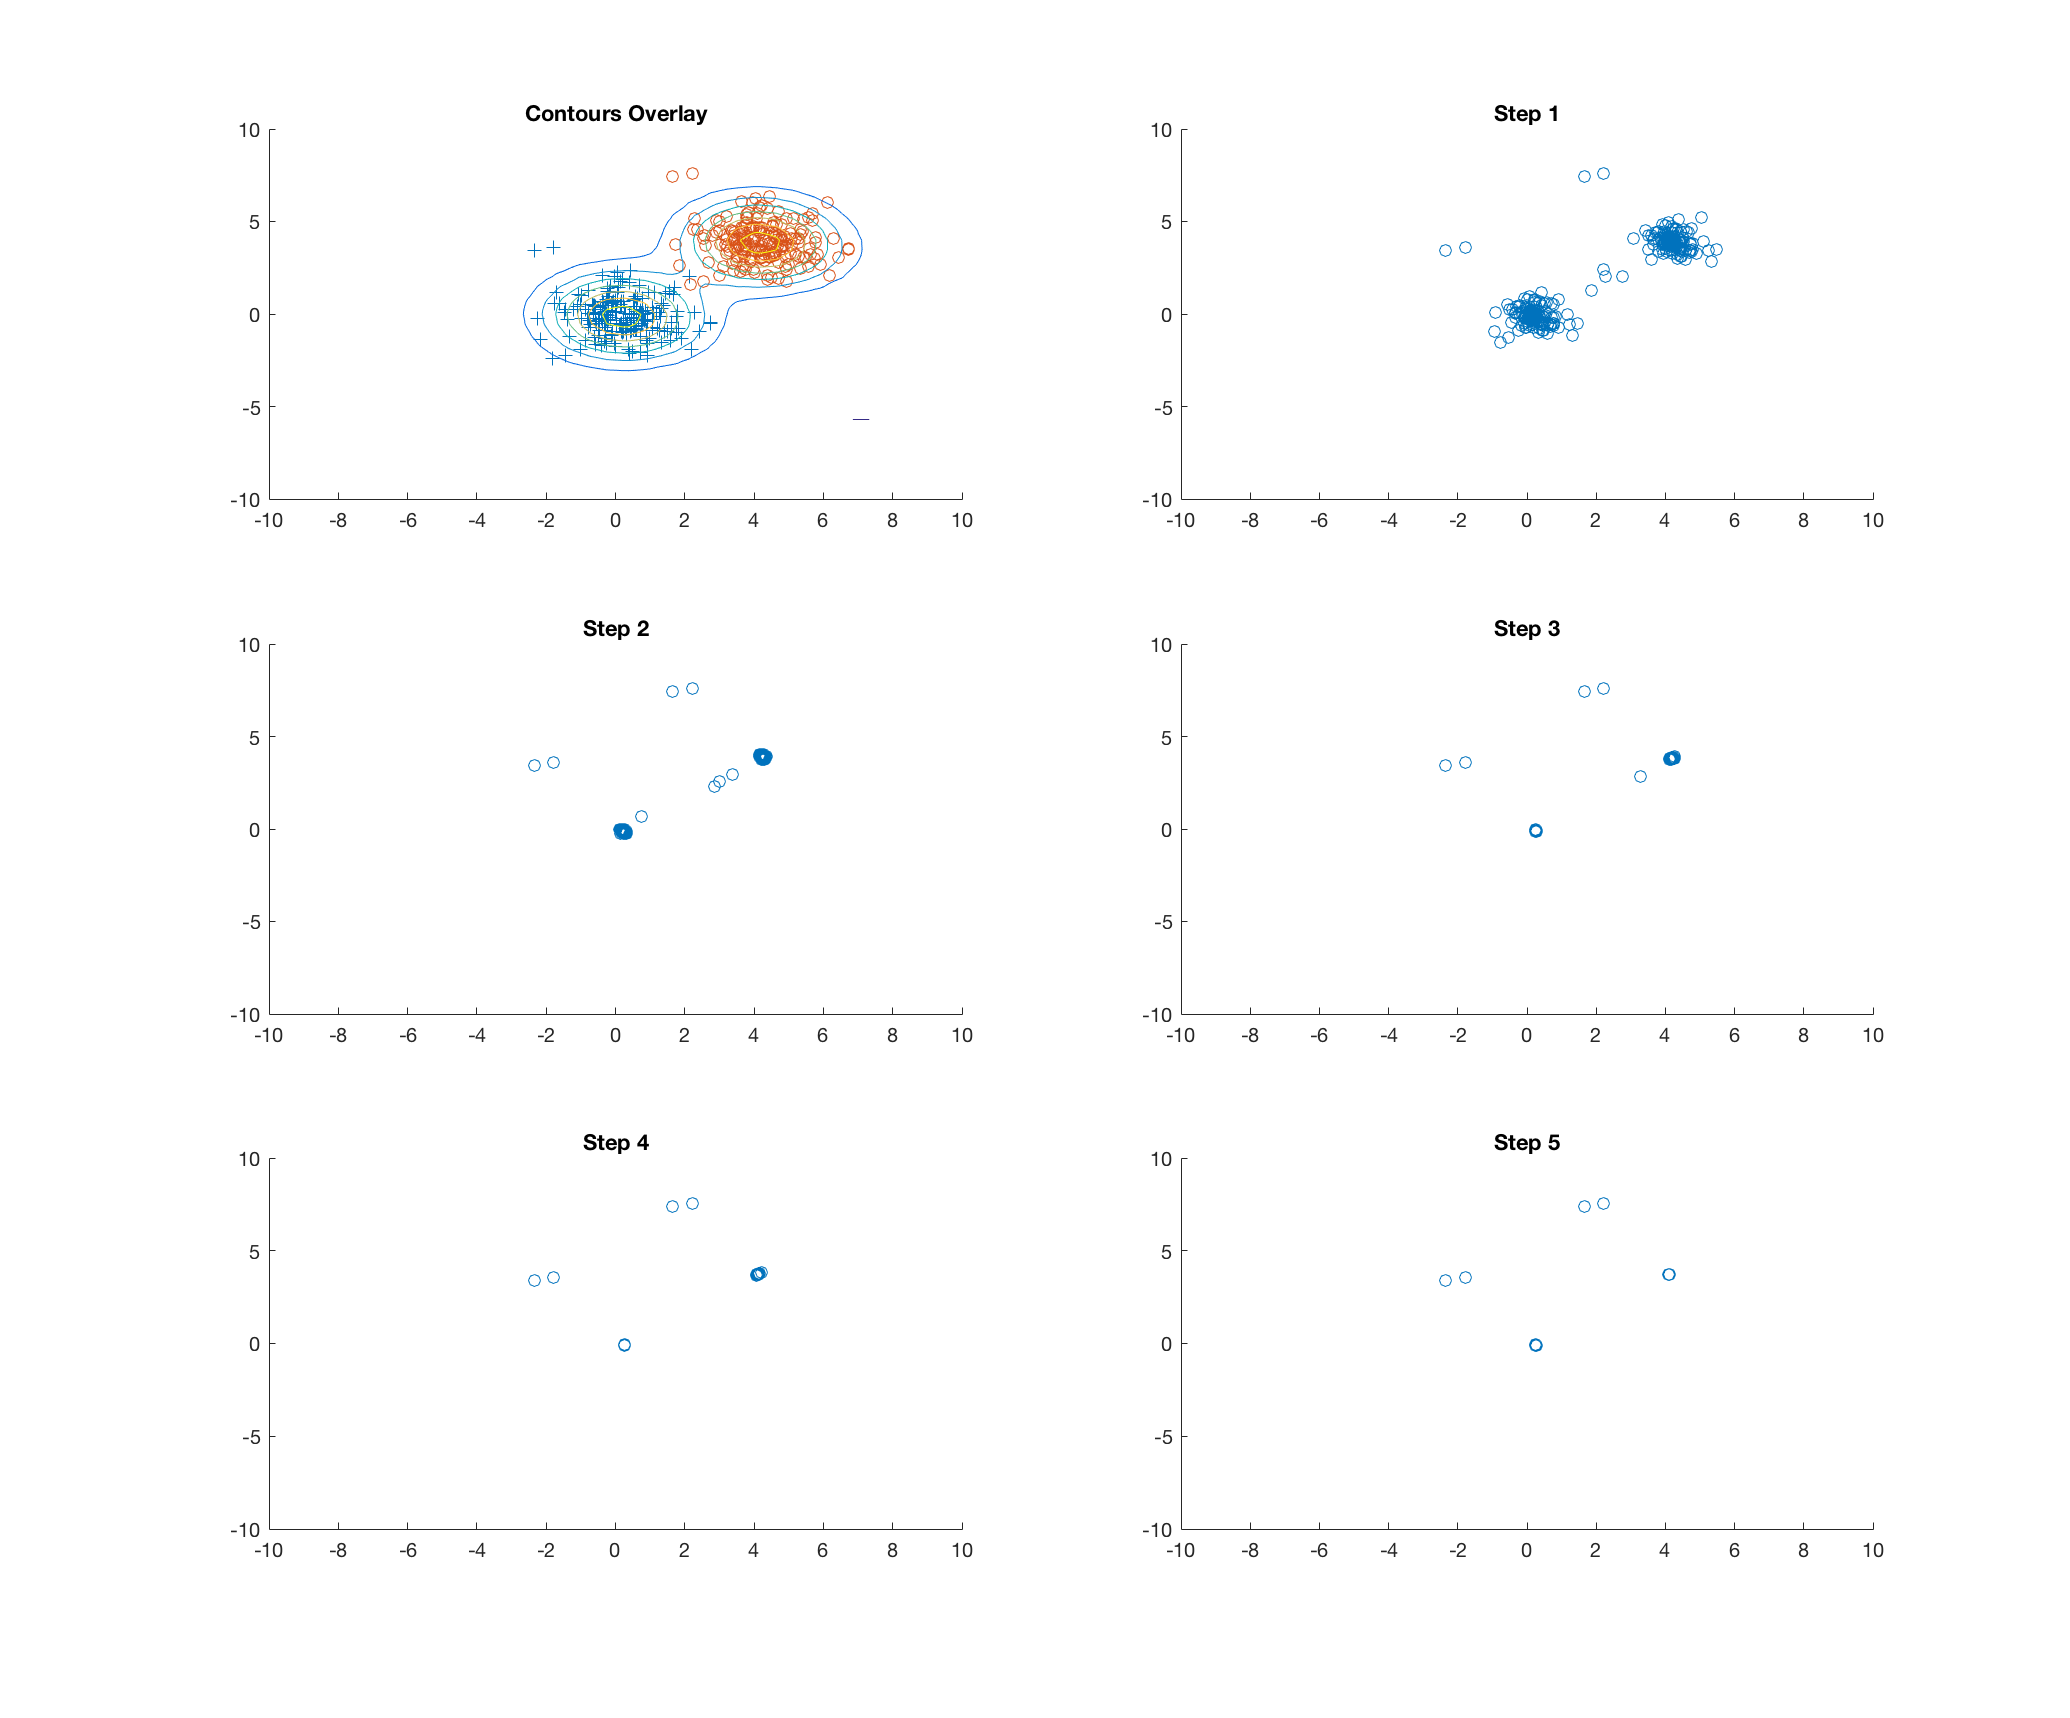
\includegraphics[width=\linewidth]{../../pracs/week5/images/q3_2class_1_8}
    \centering
    \caption{2 Classes, Lambda = 1.8}
\end{figure}

\begin{figure}[H]
    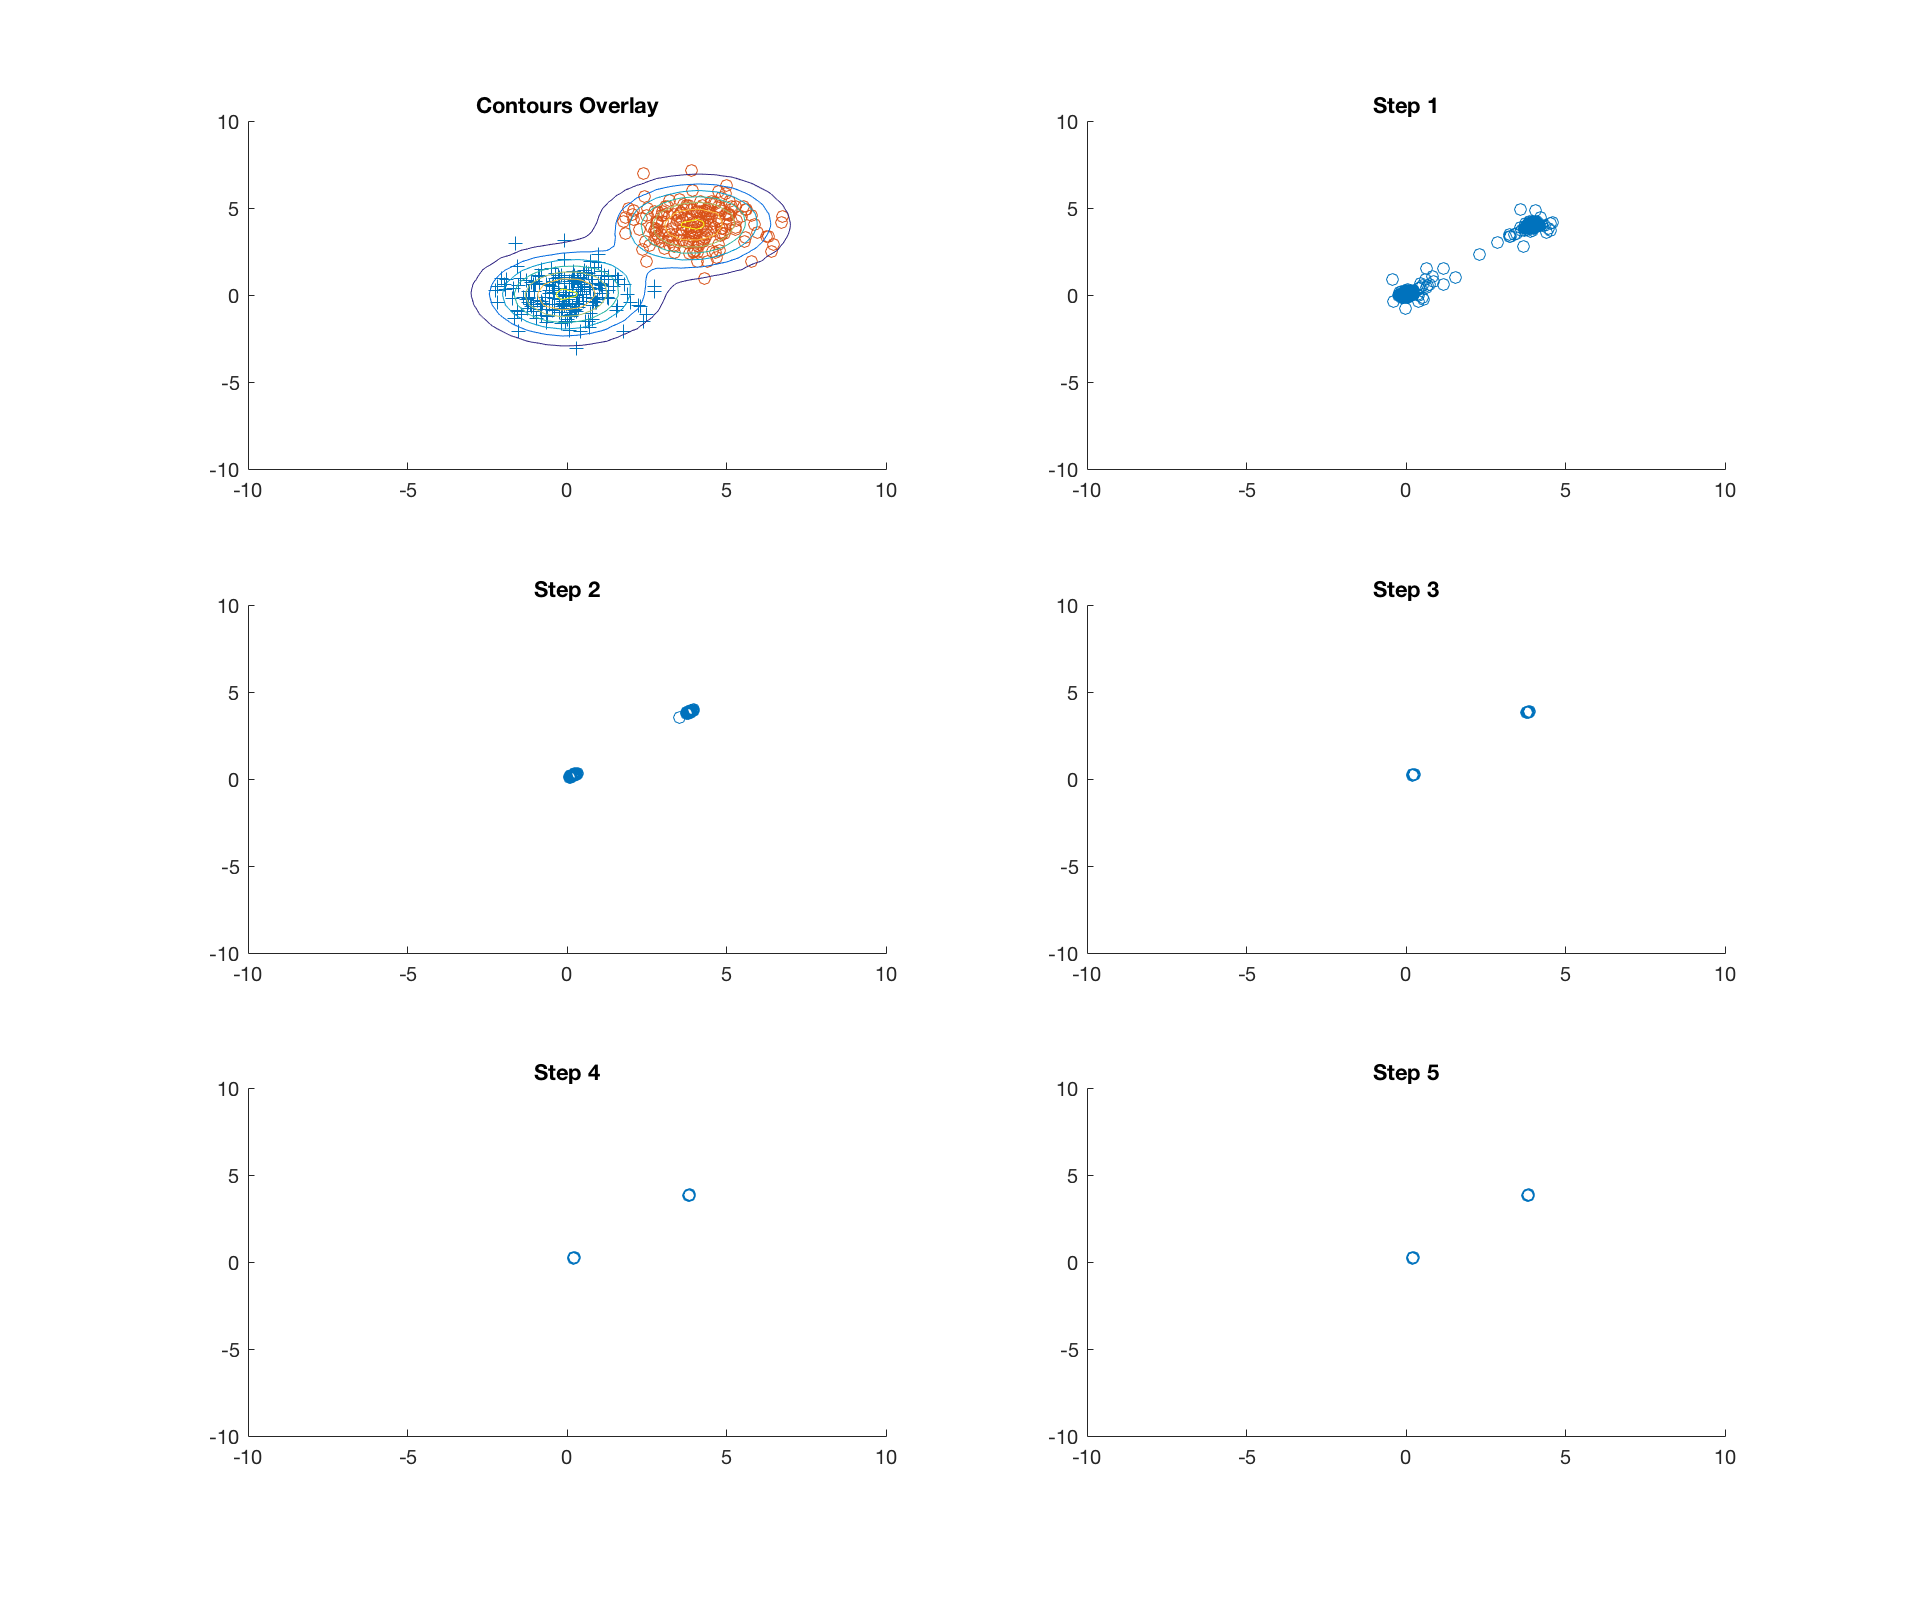
\includegraphics[width=\linewidth]{../../pracs/week5/images/q3_2class_3}
    \centering
    \caption{2 Classes, Lambda = 3}
\end{figure}

\begin{figure}[H]
    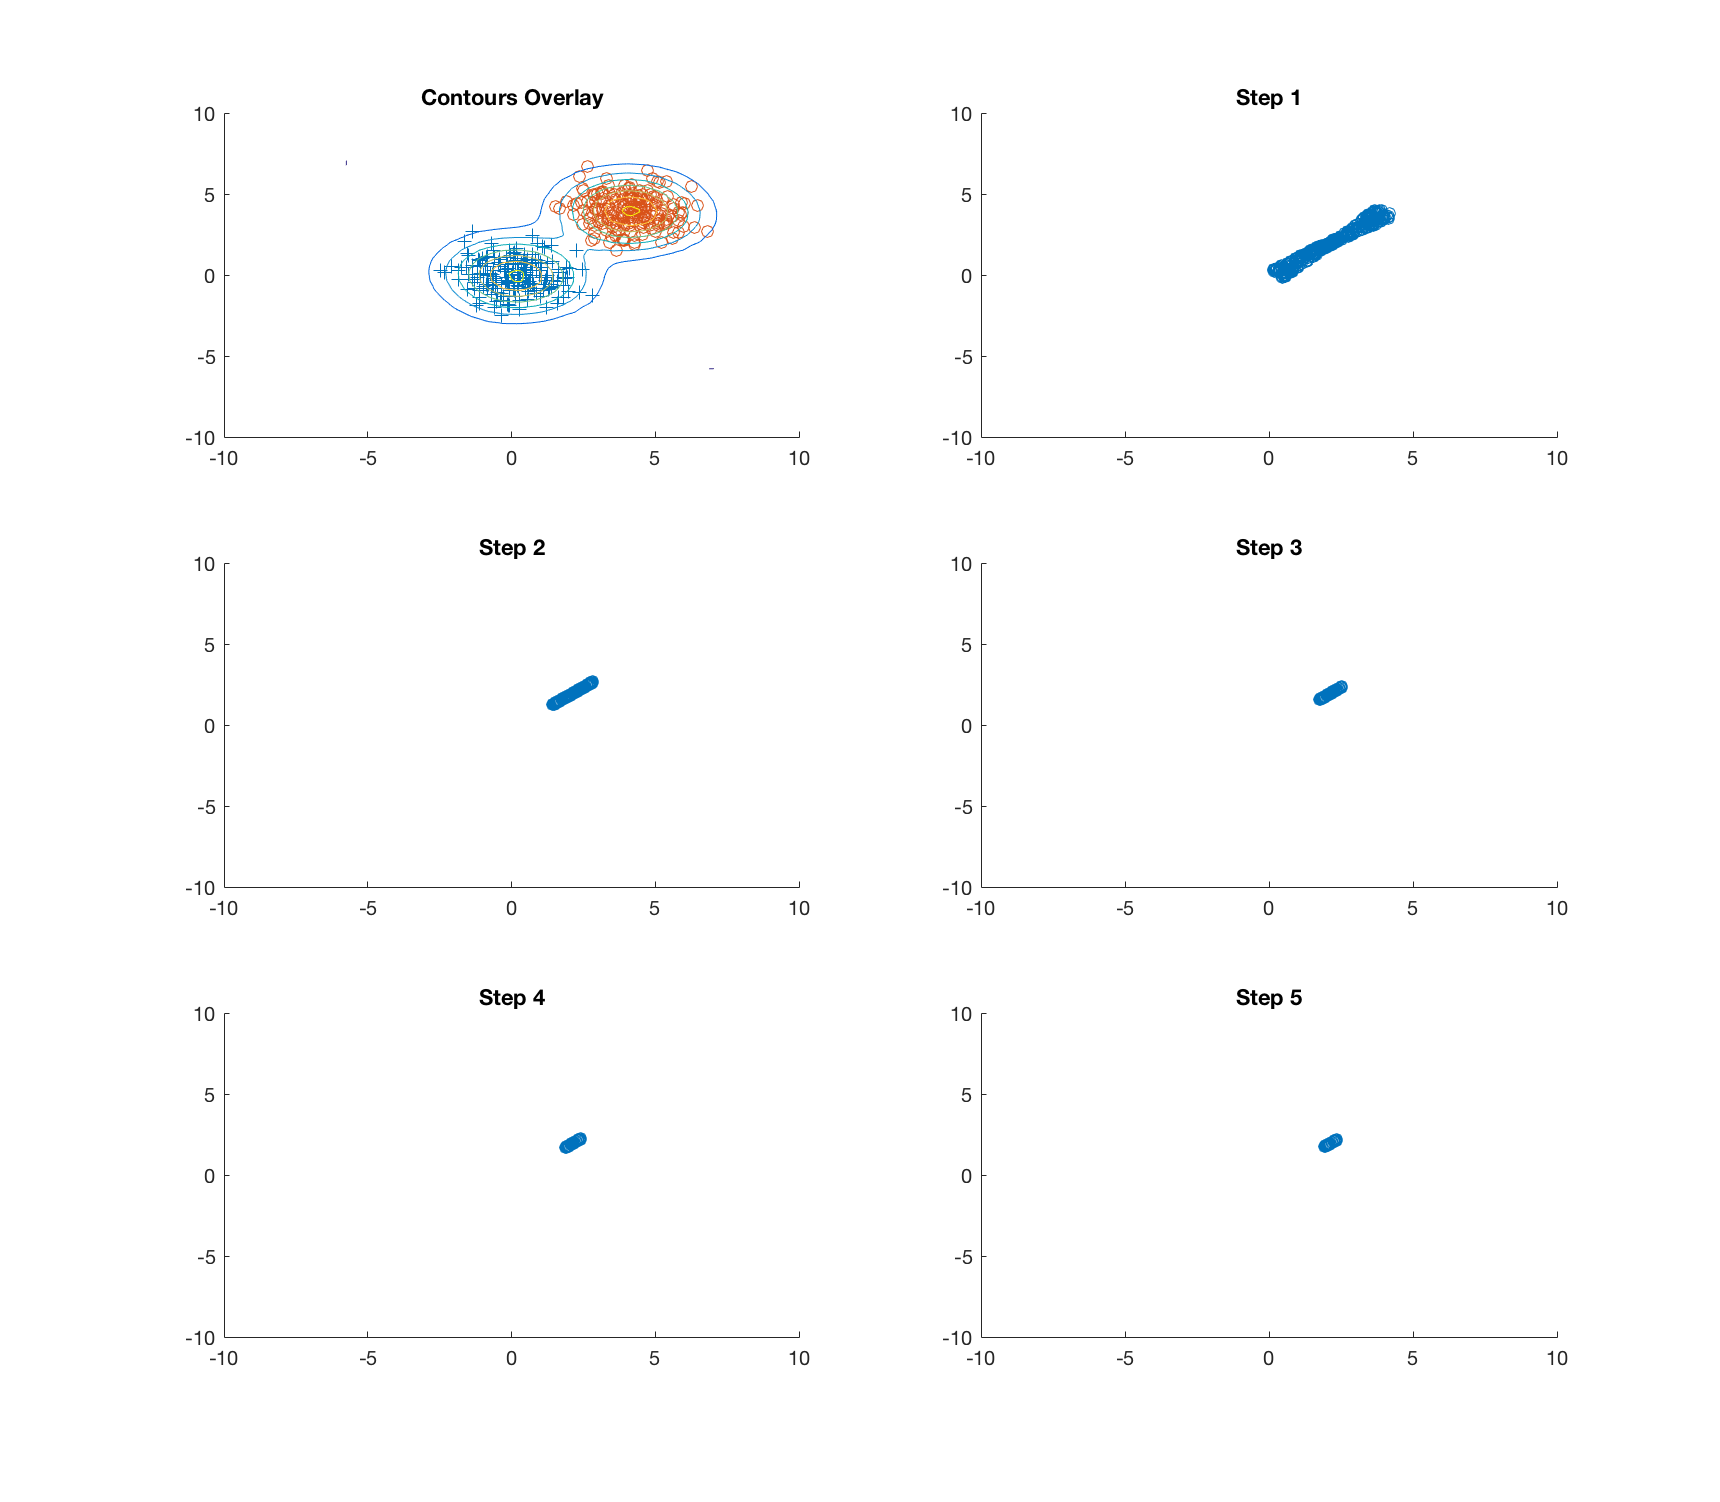
\includegraphics[width=\linewidth]{../../pracs/week5/images/q3_2class_5}
    \centering
    \caption{2 Classes, Lambda = 5}
\end{figure}

For the 2 class problem, a lambda value set to 3 provided the best result. A lambda of 1.8 cause a few outliers not to shift towards the mean value.
Whereas a lambda value of 5 caused all the points to shift towards one of the means, which is not desired.
A lambda value of 3 shifted all the points to the two mean values without leaving outliers, thus is the best lambda value out of the three.

\begin{figure}[H]
    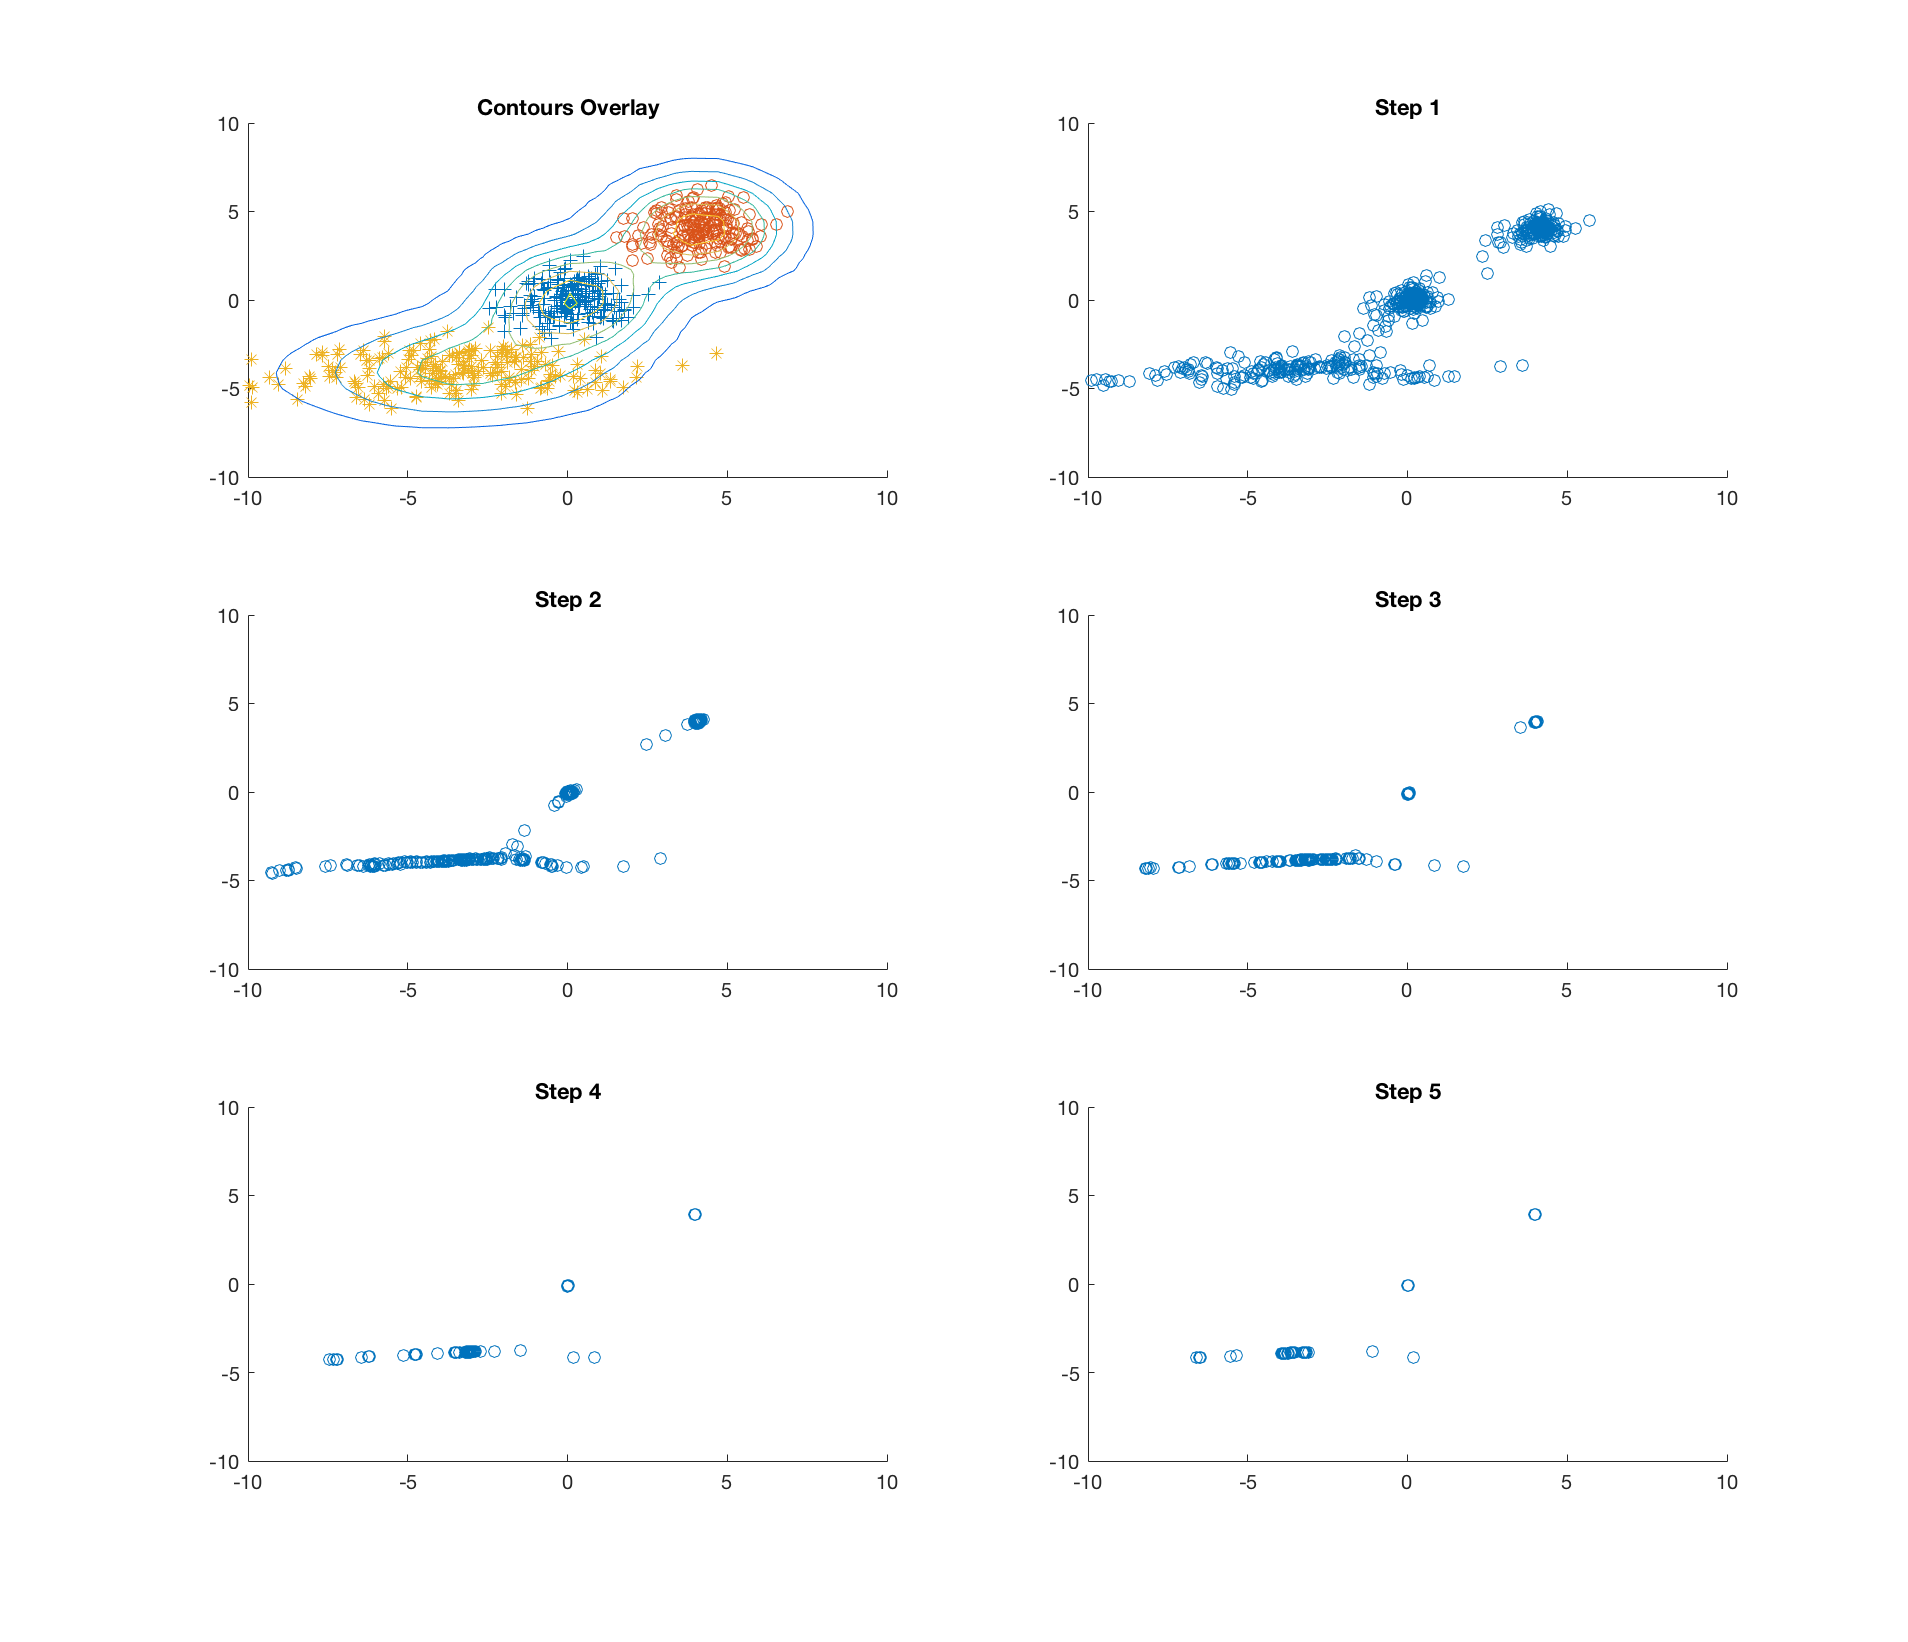
\includegraphics[width=\linewidth]{../../pracs/week5/images/q3_3class_1_8}
    \centering
    \caption{3 Classes, Lambda = 1.8}
\end{figure}

\begin{figure}[H]
    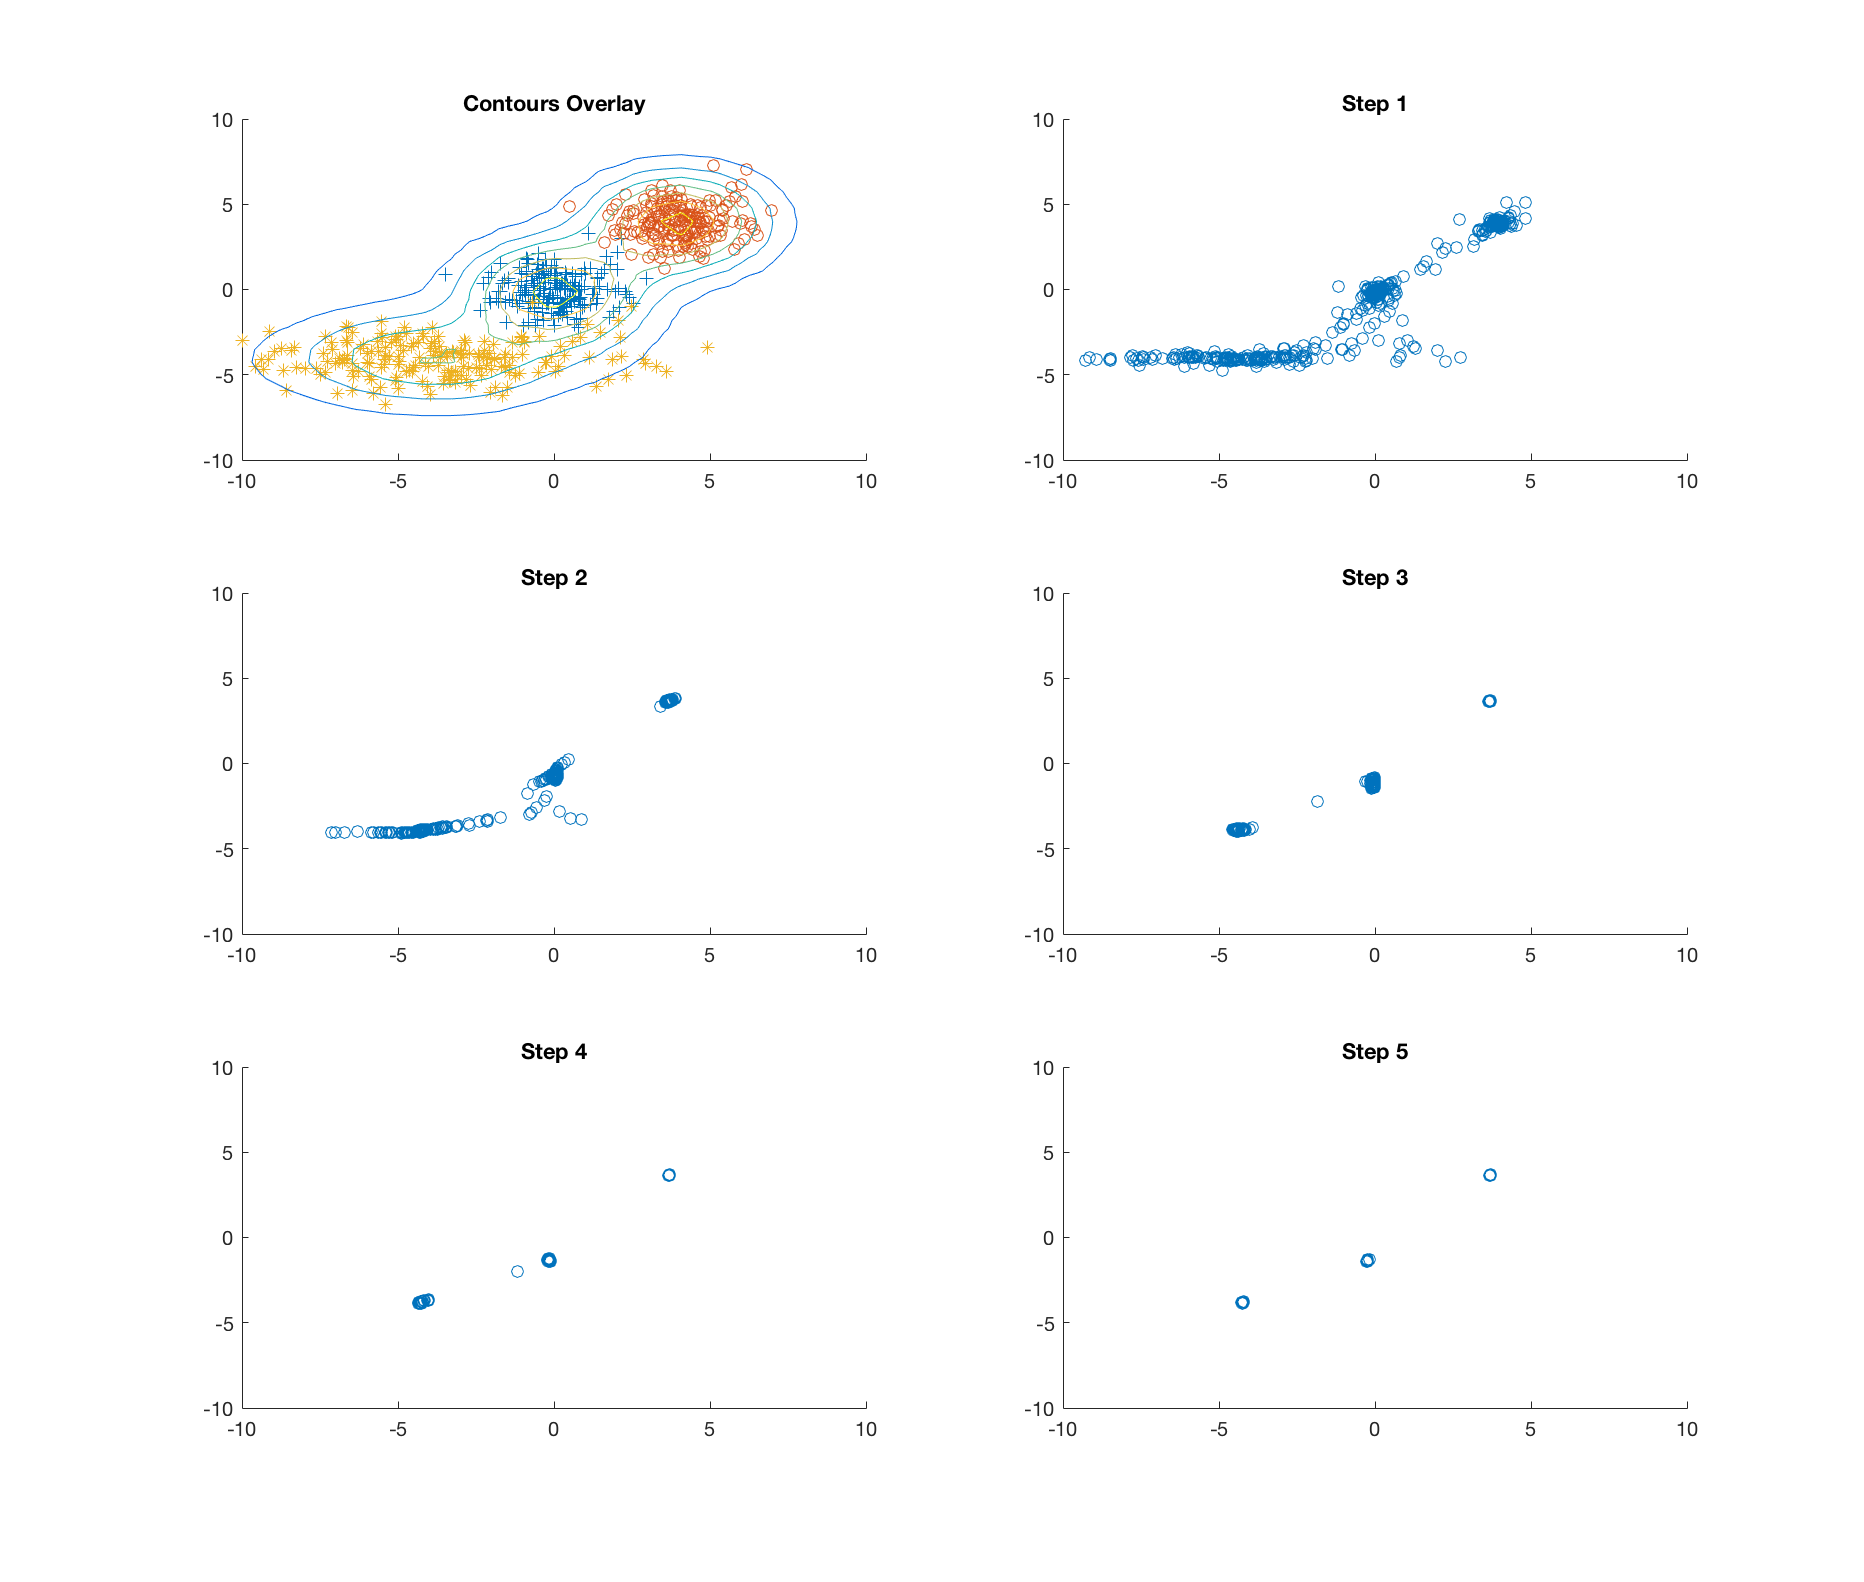
\includegraphics[width=\linewidth]{../../pracs/week5/images/q3_3class_3}
    \centering
    \caption{3 Classes, Lambda = 3}
\end{figure}

\begin{figure}[H]
    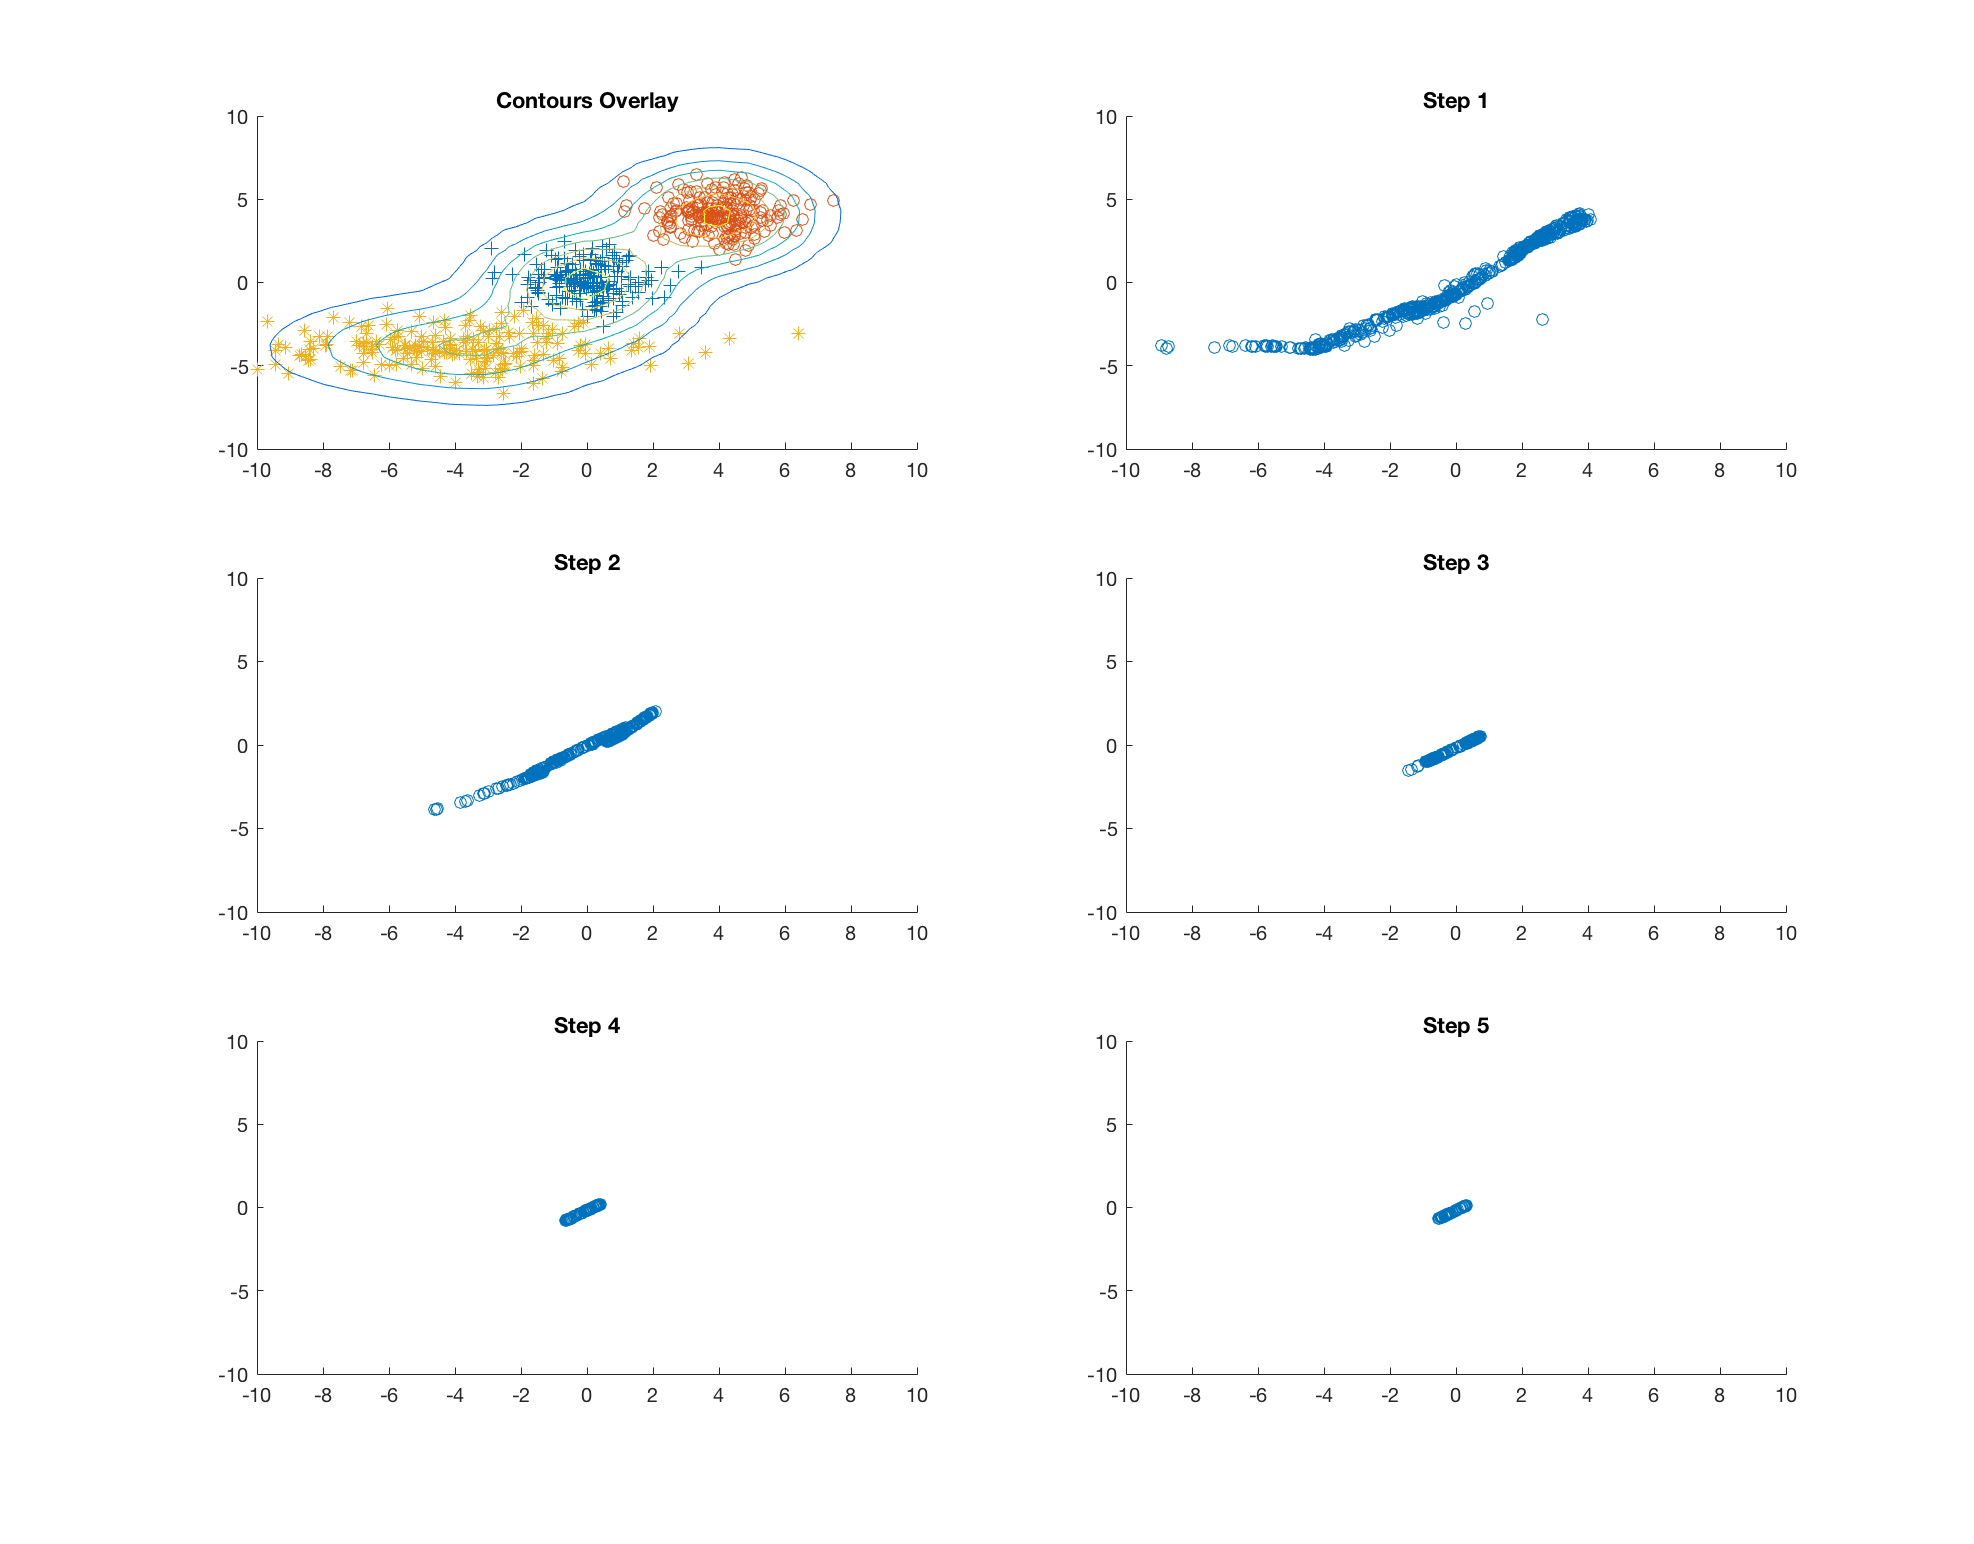
\includegraphics[width=\linewidth]{../../pracs/week5/images/q3_3class_5}
    \centering
    \caption{3 Classes, Lambda = 5}
\end{figure}

The 3 class problem showed similar results with the same lambda values 1.8, 3 and 5.
Again the 1.8 lambda value failed to shift some outliers towards the mean and the 5 lambda value shifted all of them towards a single point.
The lambda value 3 correctly shifted all the points to their respective means, thus the lambda value of 3 was the best choice out of the three numbers.

\section*{Question 5.1}

\lstinputlisting[language=Matlab]{../../pracs/week6/pca.m}

\section*{Question 5.2}

\subsection*{a}

\begin{figure}[H]
    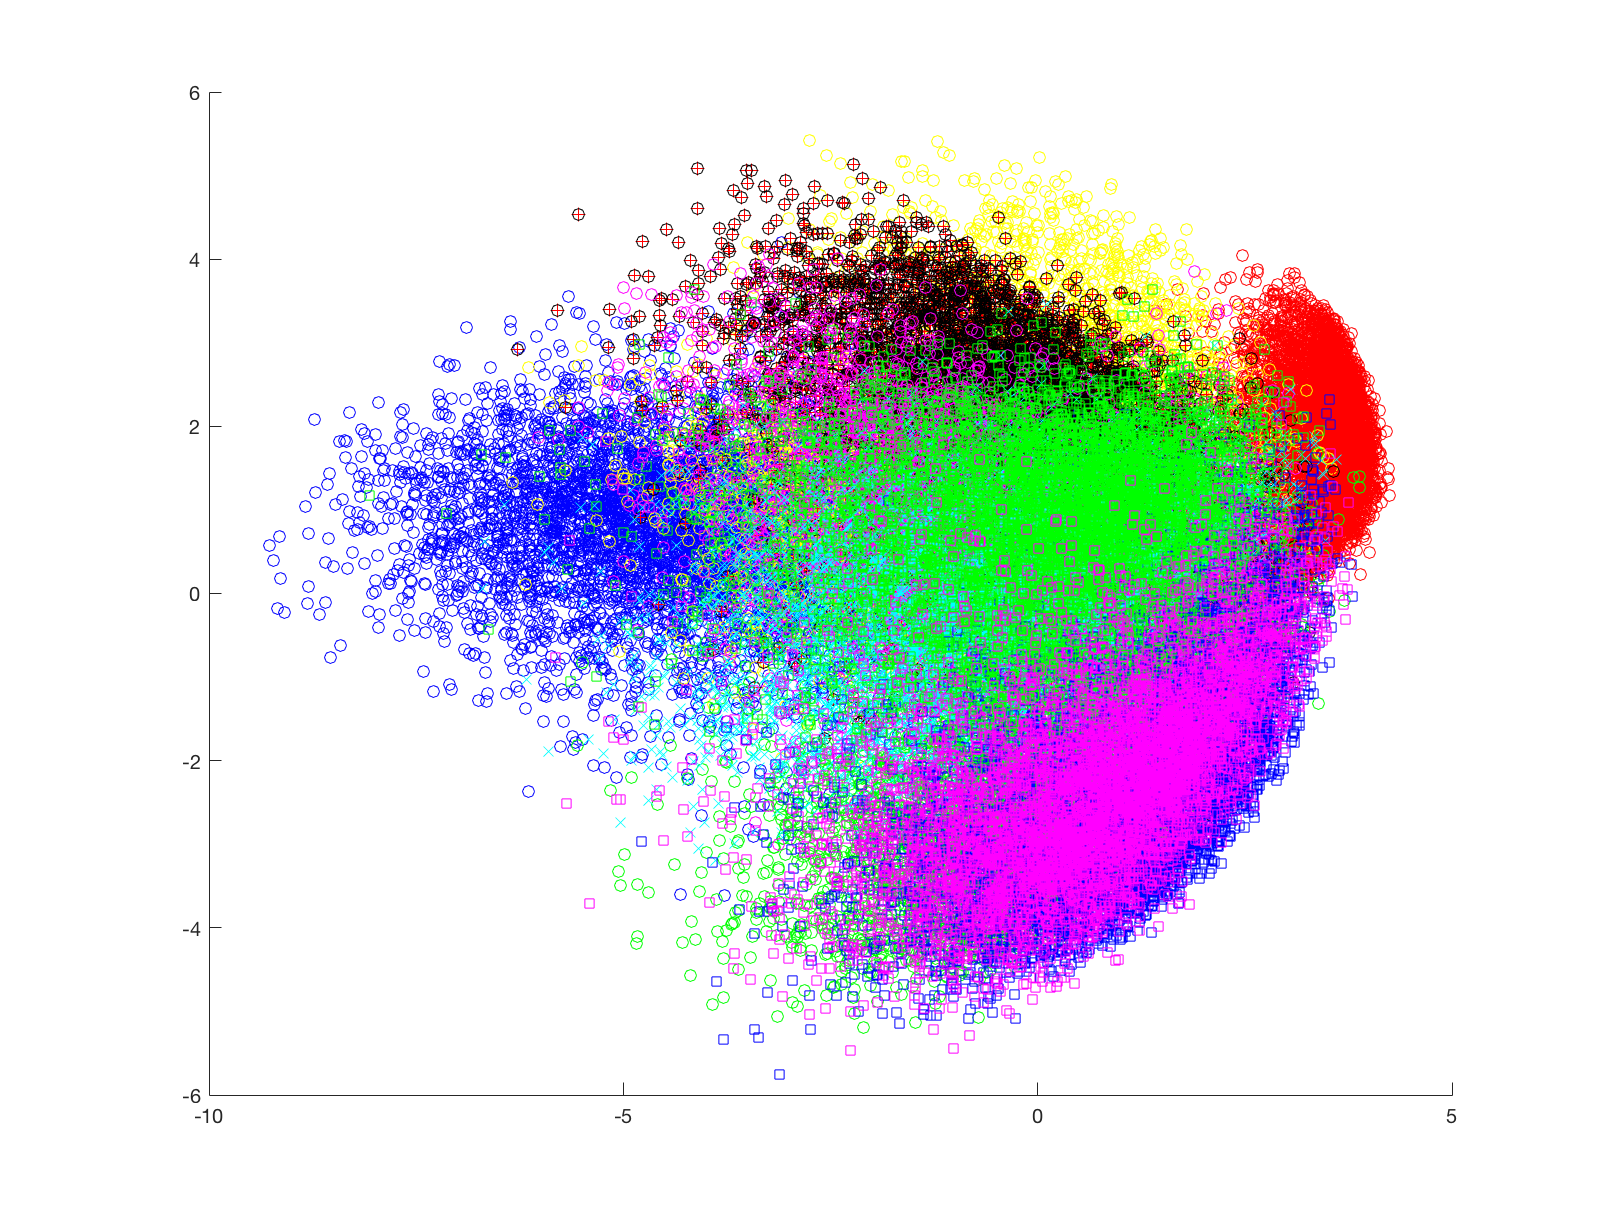
\includegraphics[width=\linewidth]{../../pracs/week6/images/q2_pca}
    \centering
    \caption{PCA on MNIST dataset}
\end{figure}

\subsection*{b}

The first principle component accounts for 5.116\% of the data, whereas the second principle component accounts for 3.7414\% of the data.

\subsection*{c}

\begin{figure}[H]
    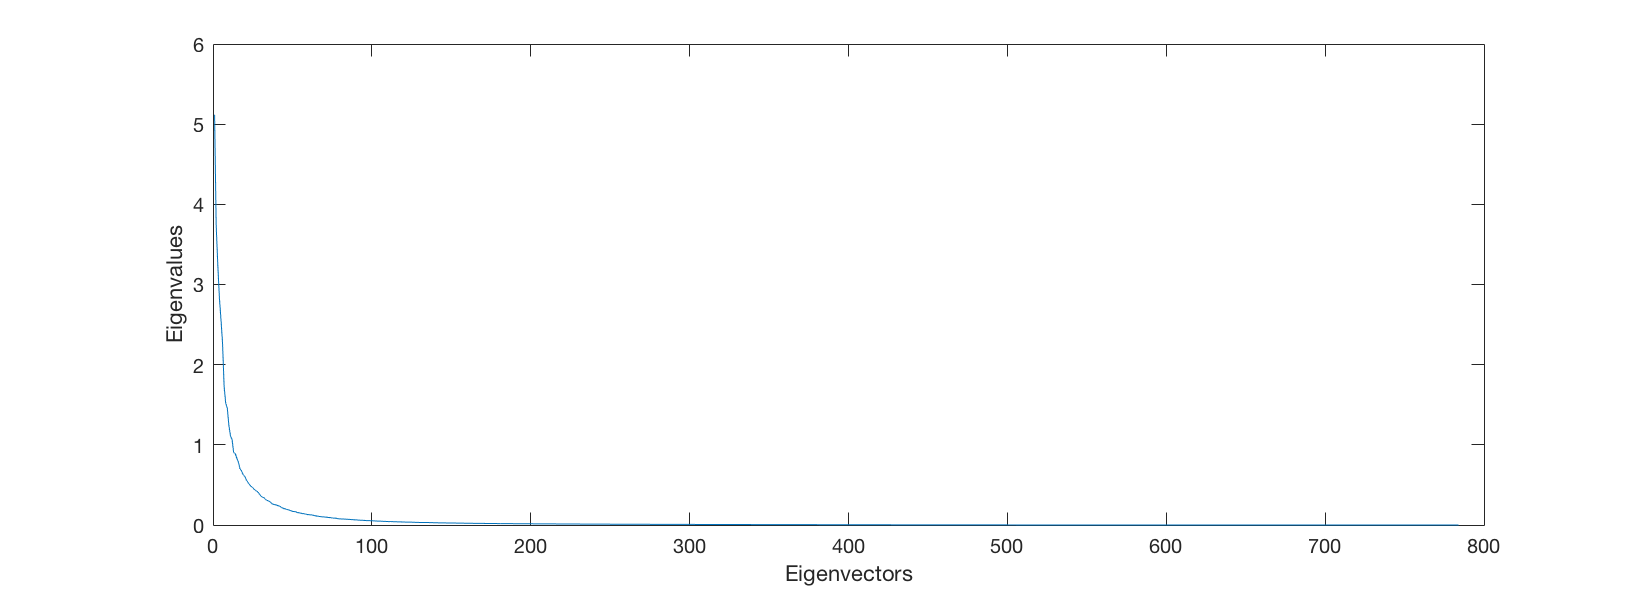
\includegraphics[width=\linewidth]{../../pracs/week6/images/scree_graph}
    \centering
    \caption{Scree Graph}
\end{figure}

\section*{Question 5.6}

\begin{figure}[H]
    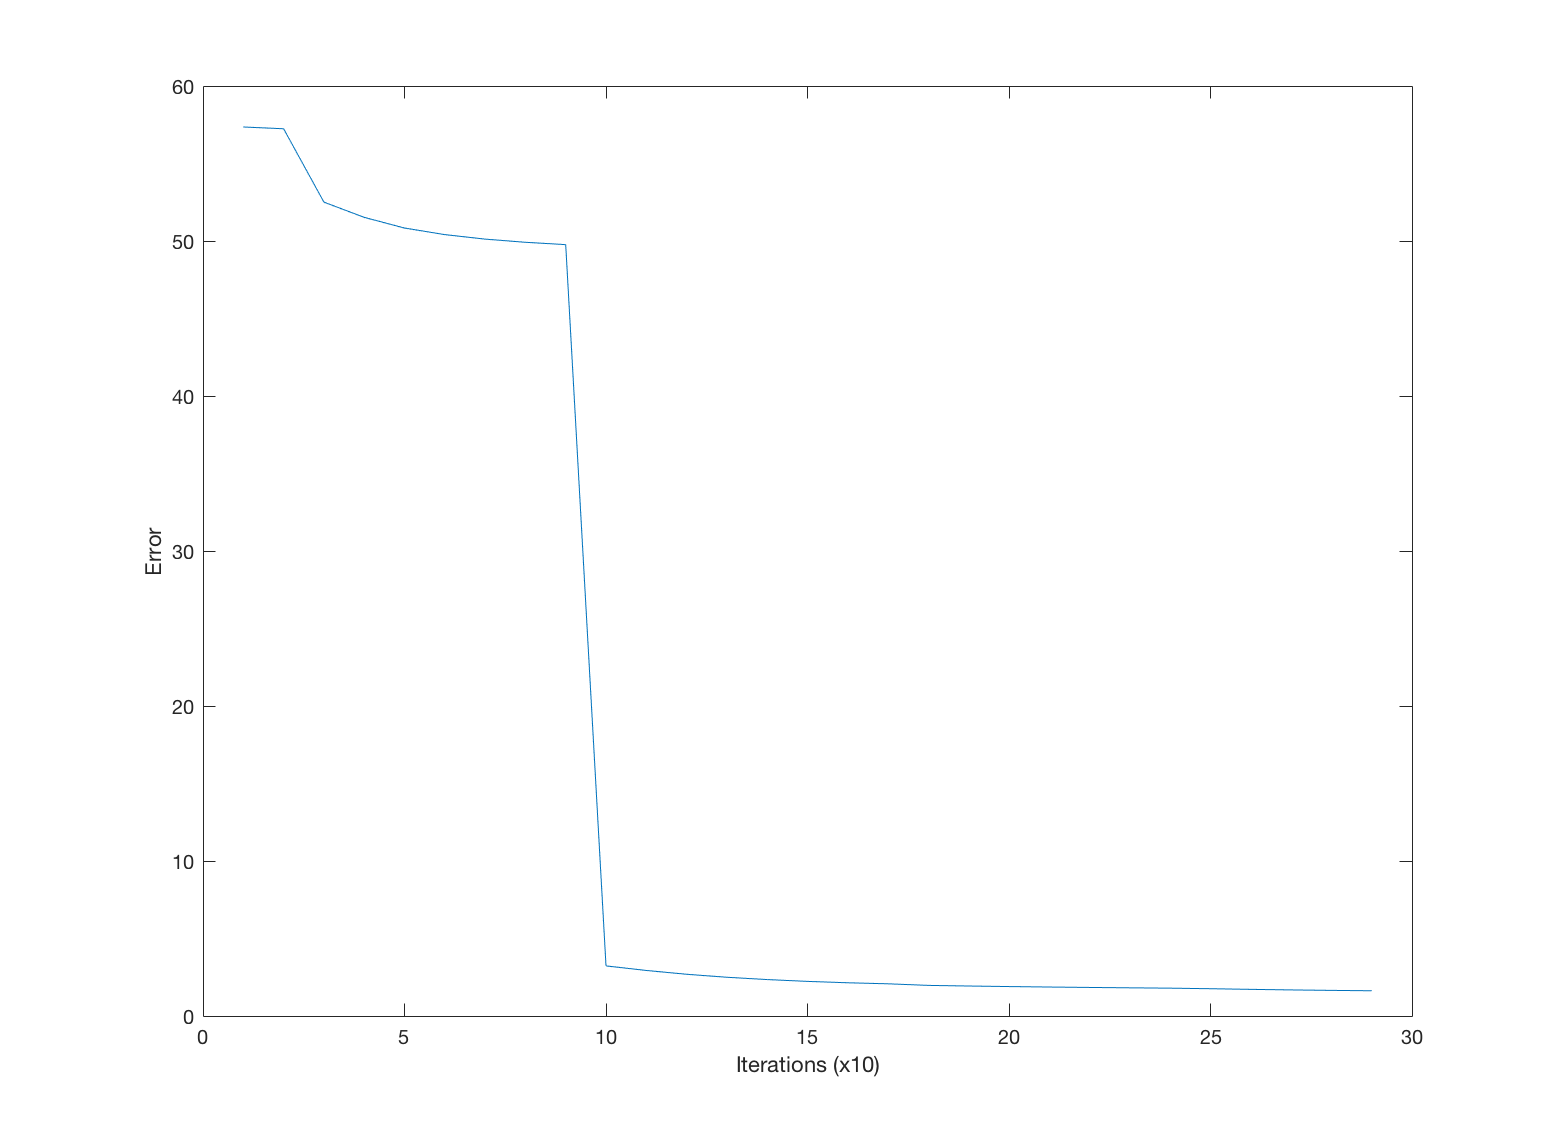
\includegraphics[width=\linewidth]{../../pracs/week6/images/q6_error}
    \centering
    \caption{Error vs Iteration}
\end{figure}

\begin{figure}[H]
    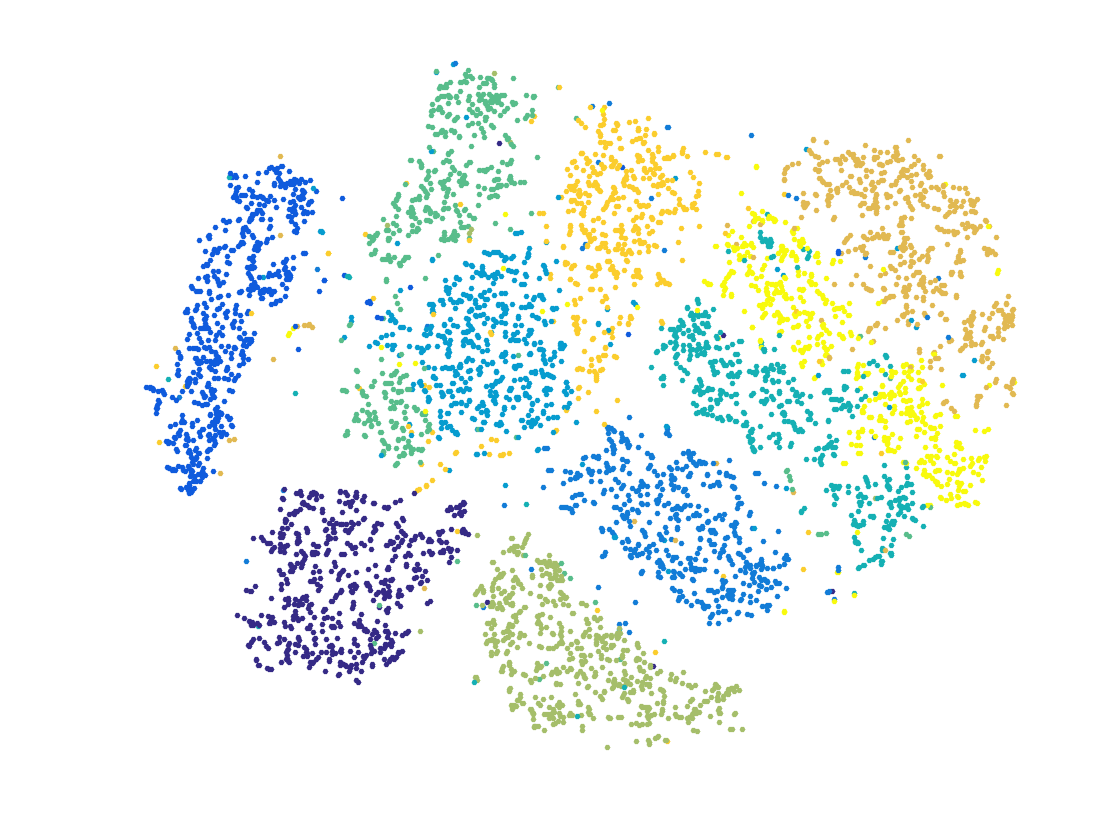
\includegraphics[width=\linewidth]{../../pracs/week6/images/q6}
    \centering
    \caption{Iteration 300}
\end{figure}

\section*{Question 5.8}

\begin{figure}[H]
    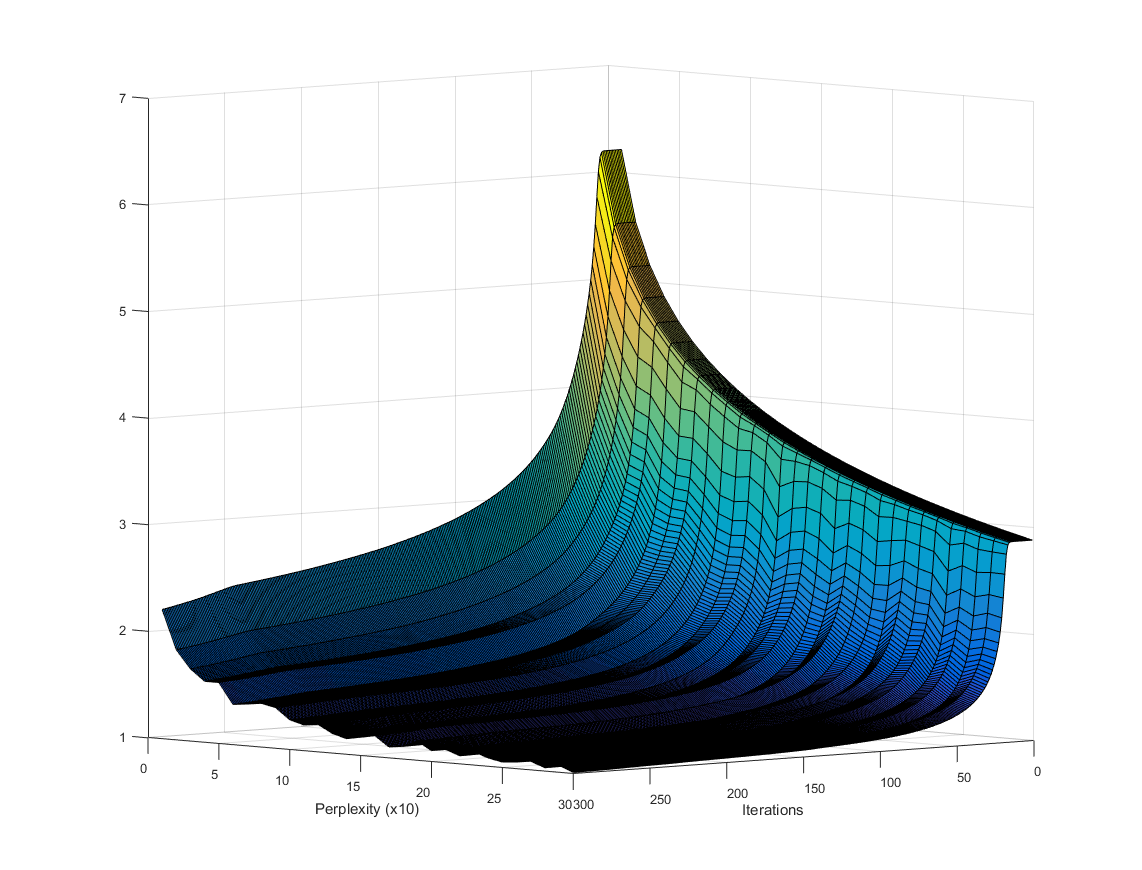
\includegraphics[width=\linewidth]{../../pracs/week6/images/q8}
    \centering
    \caption{Perplexity and Iterations on Cost}
\end{figure}

The perplexity determines how to balance the attention between local and global aspects of the dataset.
The graph shows the error change on iterations, thus we should choose a perplexity the reduces the error as quickly as possible, such that the algorithm requires less iterations to find a good solution.
A simple heuristic to choose a good perplexity would be to look for the greatest rate of change in the error, by inspecting the chart we can see that the lower perplexities have far greater rate of change.
Further inspection showed that a perplexity value of 2 provided the best rate of change.

\begin{figure}[H]
    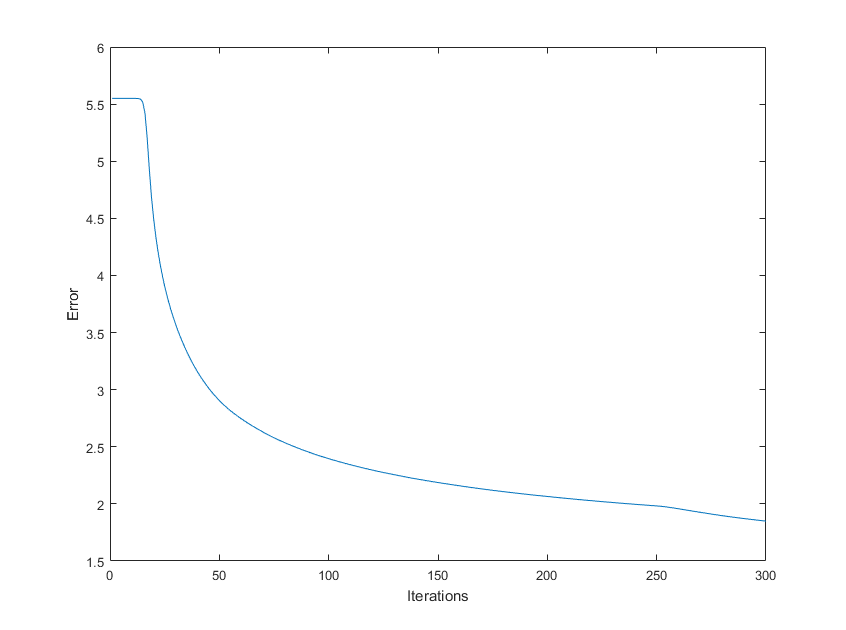
\includegraphics[width=\linewidth]{../../pracs/week6/images/q8_p2}
    \centering
    \caption{Error on Perplexity}
\end{figure}

\end{document}
